\chapter{线性代数}
    \section{矩阵}
    一个$m\times n$矩阵(matrix)就是一个有$m$行$n$列的数表:
    \begin{equation}
        \label{eq:1}
        \bm{A}=
        \mqty(
            a_{11} & a_{12} & \cdots & a_{1n} \\
            a_{21} & a_{22} & \cdots & a_{2n} \\
            \vdots & \vdots & \ddots & \vdots \\
            a_{m1} & a_{m2} & \cdots & a_{mn} \\
        )
    \end{equation}

    如果$m=n$(行数等于列数),这样的矩阵就是正方形的,叫做方阵。方阵可以定义行列式(determinant)$|\bm{A}|$。
    \begin{equation}
        \label{eq:2}
        |\bm{A}|=
        \mqty|
            a_{11} & a_{12} & \cdots & a_{1n} \\
            a_{21} & a_{22} & \cdots & a_{2n} \\
            \vdots & \vdots & \ddots & \vdots \\
            a_{n1} & a_{n2} & \cdots & a_{nn} \\
        |
    \end{equation}

    对于方阵,可以定义她的转置$\bm{A}'$:
    \begin{equation}
        \label{eq:3}
        \bm{A}'=
        \mqty(
            a_{11} & a_{21} & \cdots & a_{n1} \\
            a_{12} & a_{22} & \cdots & a_{n2} \\
            \vdots & \vdots & \ddots & \vdots \\
            a_{1n} & a_{2n} & \cdots & a_{nn} \\
        )
    \end{equation}

    行列式有如下的性质:
    \begin{enumerate}
        \item 方阵转置前后,行列式不变\footnote{这意味着行列式的对行成立的性质对列也成立。所以接下来我们就只叙述行的情况};
        \item 对换任意两行,行列式改变符号;
        \item 行列式两行成比例(或相等),则行列式为零;
        \item 以其中一行的某个倍数加到另一行上,行列式值保持不变;
        \item 如果其中一行可以拆成两项之和,则行列式可以按这两项拆成两个行列式之和;
        \item 上(下)三角行列式的值等于主对角元素的乘积;
        \item 将行列式的某行乘以$c$倍,则新行列式的值等于原行列式的$c$倍;
    \end{enumerate}

    行列式$|\bm{A}|$的第$(i,j)$元素$a_{ij}$的余子式$M_{ij}$是指划掉了$a_{ij}$所在的那一行和那一列之后,剩下的所有元素保持相对位置不动组成的新的低一阶的行列式。代数余子式$A_{ij}=(-1)^{i+j}M_{ij}$,也就是余子式带上一个符号。Laplace定理说的是:行列式$|\bm{A}|$可以按照任意一行或任意一列进行展开,且形式如下(按第$r$行、第$l$列进行展开):
    \begin{equation}
        \label{eq:4}
        |\bm{A}|=\sum_{i=1}^{n}a_{ri}A_{ri}=\sum_{i=1}^{n}a_{il}A_{il}
    \end{equation}

    证明就省略了。

    \section{矩阵的运算}
    矩阵之间可以定义加法,取自数域$\mathbb{F}$的数乘和矩阵间的乘法。设$\bm{A}=(a_{ij})_{m\times n}$,$\bm{B}=(b_{ij})_{m\times n}$,则矩阵间的加法是
    \begin{equation}
        \label{eq:5}
        \bm{A}+\bm{B}=(a_{ij}+b_{ij})_{m\times n}
    \end{equation}
    
    设$C\in\mathbb{F}$,则
    \begin{equation}
        \label{eq:6}
        C\bm{A}=(Ca_{ij})_{m\times n}
    \end{equation}

    两个相同形状的矩阵$\bm{A},\bm{B}$之间的减法$\bm{A}-\bm{B}$定义为$\bm{A}+(-\bm{B})$。其中$-\bm{B}$是$\bm{B}$的负矩阵。


    两个矩阵$\bm{A}=(a_{ij})_{m\times n},\bm{B}=(b_{ij})_{s\times t}$相等的充分必要条件是$m=s,n=t$且$a_{ij}=b_{ij}$。

    矩阵的乘法是这样定义的:设$\bm{A}$是一个$m\times s$矩阵,$\bm{B}$是一个$s\times n$矩阵,乘积$\bm{C}=\bm{A}\bm{B}$是一个$m\times n$矩阵,且$\bm{C}$的第$(i,j)$元素定义为:
    \begin{equation}
        \label{eq:7}
        c_{ij}=\sum_{k=1}^{s}a_{ik}b_{kj}
    \end{equation}

    \begin{figure}[htbp]
        \begin{center}
            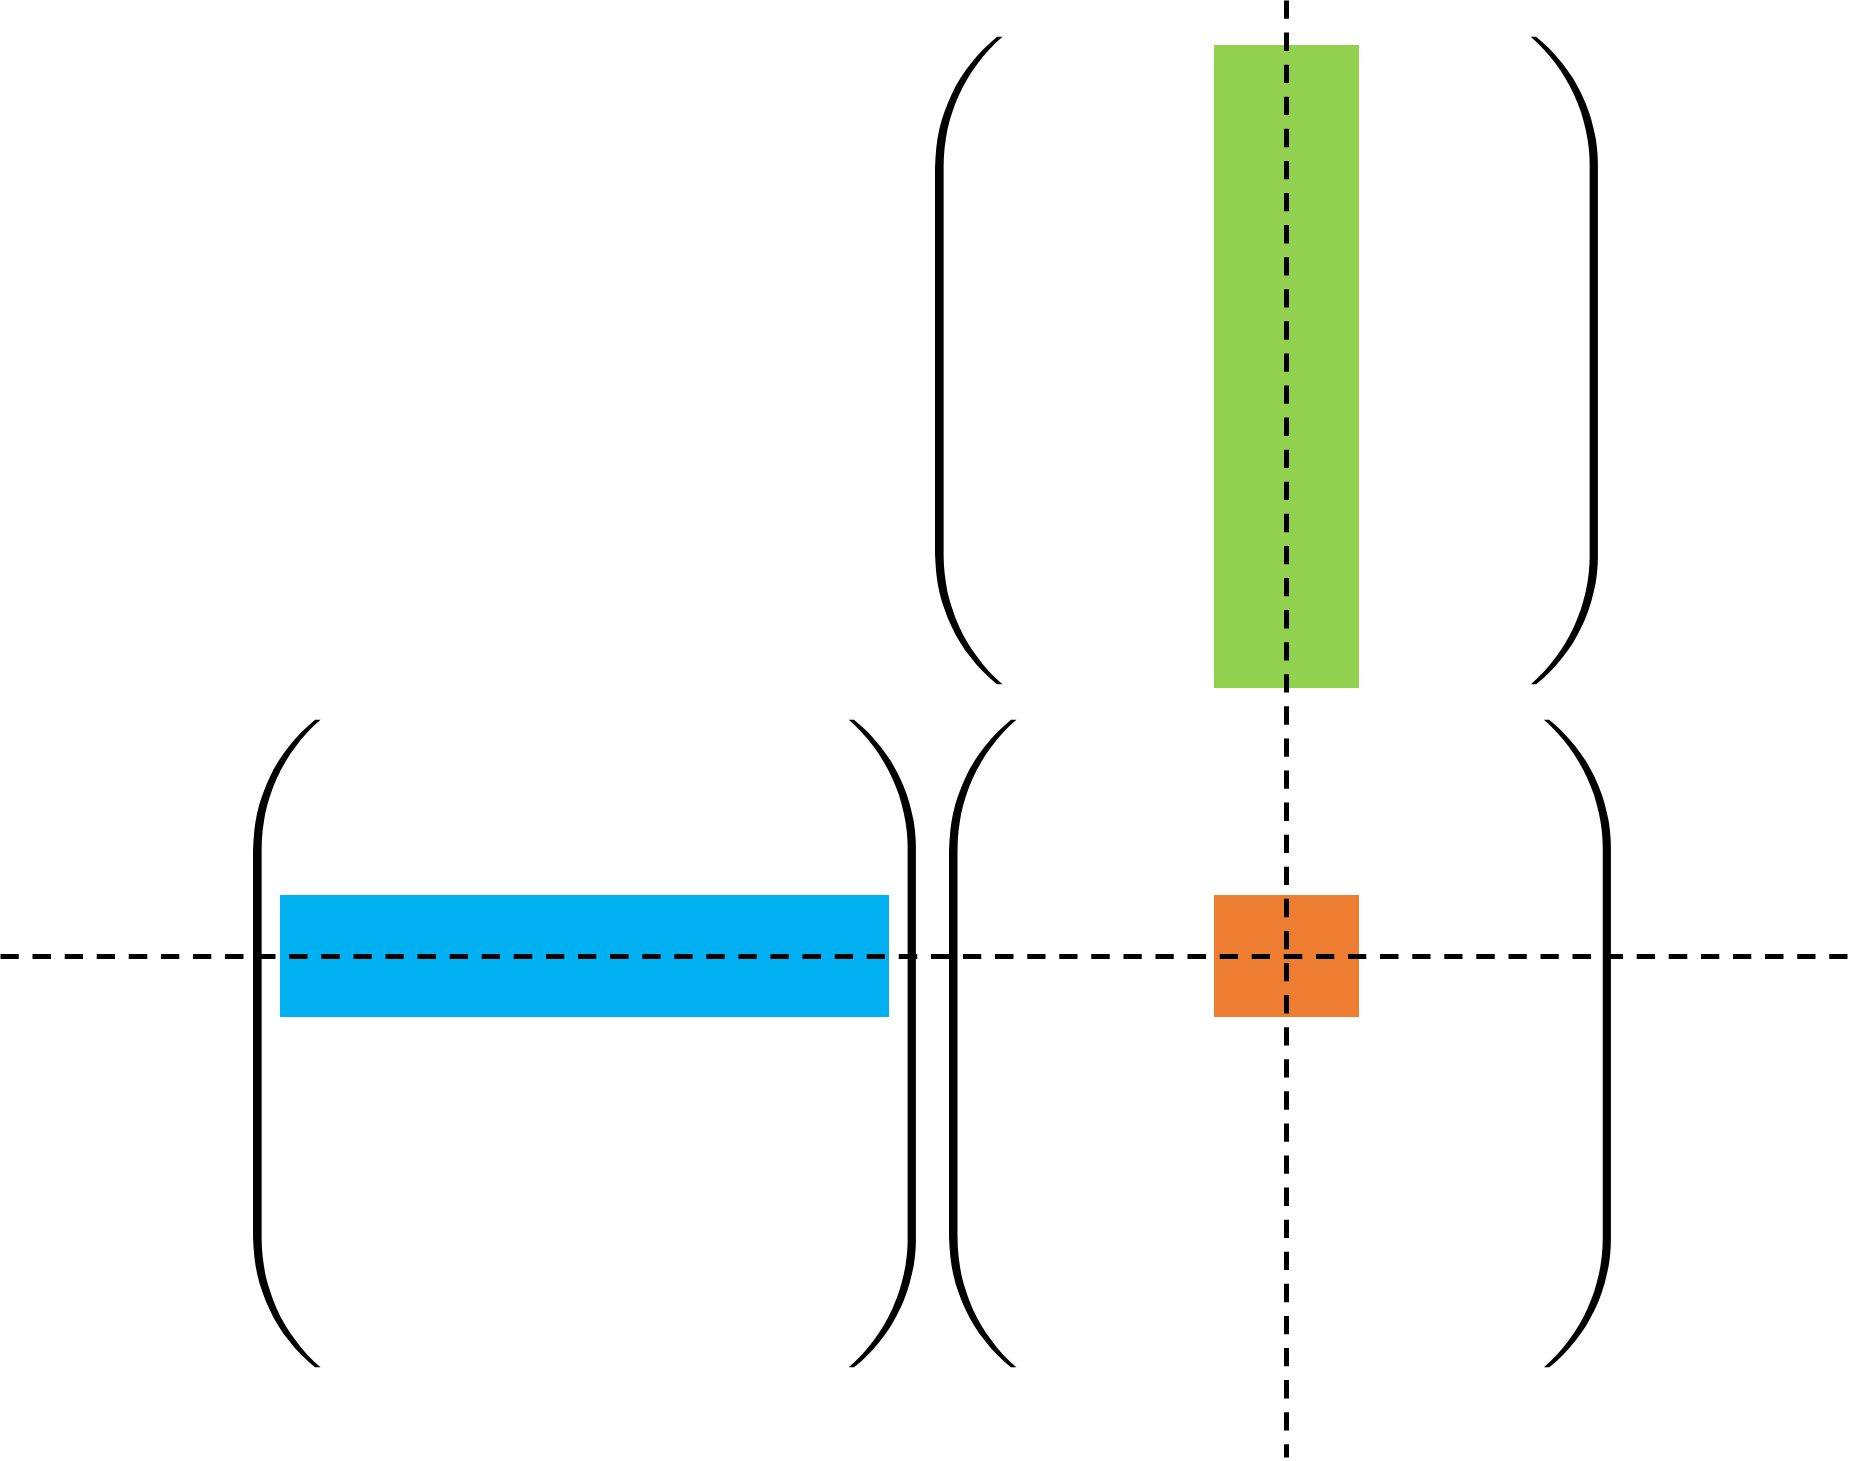
\includegraphics[scale=0.5]{imgs/img1.png}
        \end{center}
        \caption{阵矩乘法可视化}
        \label{fig:1}
    \end{figure}

    \ref{fig:1}演示了矩阵相乘的规则,也就是左边矩阵取第$i$行,右边矩阵取第$j$列,然后按求和指标$k$逐项相乘后再相加,最后的和就是乘积的第$(i,j)$元素$c_{ij}$。图片\ref{fig:1}中展示了一种快速记忆矩阵乘法规则的方式:把右边的矩阵向上抬,然后左边矩阵、右边矩阵分别向右侧、下侧划线$l_1,l_2$,$l_1,l_2$的交点代表乘积的第$(i,j)$元素,$l_1$从左至右会和左边矩阵交于$a_{ik},k=1,2,\cdots,s$这些矩阵元,$l_2$从上至下会和右边矩阵交于$b_{kj},k=1,2,\cdots,s$这些矩阵元,依相交时的次序两两相乘再相加,就可以得到$c_{ij}$这个矩阵元。

    最后我们强调:绝大多数矩阵之间的乘积是不可交换的,也就是$\bm{A}\bm{B}\ne\bm{B}\bm{A}$。因此在一些学科中会引入交换子(commutator)$[\bm{A},\bm{B}]$来描述两个矩阵乘积不可交换的程度。具体而言就是交换位置相乘再相减。
    \begin{equation}
        \label{eq:8}
        [\bm{A},\bm{B}]=\bm{A}\bm{B}-\bm{B}\bm{A}
    \end{equation}
    
    我们在这里给出矩阵运算的一些性质和这些性质的证明过程:
    \begin{enumerate}
        \item 加法交换律:$\bm{A}+\bm{B}=\bm{B}+\bm{A}$;
        \item 加法结合律:$\bm{A}+(\bm{B}+\bm{C})=(\bm{A}+\bm{B})+\bm{C}$;
        \item 对数乘的交换律:$k(l\bm{A})=(kl)\bm{A}$;
        \item 加法对数乘的分配律:$c(\bm{A}+\bm{B})=c\bm{A}+c\bm{B}$;
        \item 乘法结合律:$\bm{A}(\bm{B}\bm{C})=(\bm{A}\bm{B})\bm{C}$;
        \item 乘法分配律:$\bm{A}(\bm{B}+\bm{C})=\bm{A}\bm{B}+\bm{A}\bm{C}$,$(\bm{A}+\bm{B})\bm{C}=\bm{A}\bm{C}+\bm{B}\bm{C}$;
        \item $c(\bm{A}\bm{B})=(c\bm{A})\bm{B}=\bm{A}(c\bm{B})$。
    \end{enumerate}

    \begin{proof}
        根据数字加法的交换律易证。
    \end{proof}

    \begin{proof}
        根据数字加法的结合律易证。
    \end{proof}

    \begin{proof}
        根据数字乘法的交换律易证。
    \end{proof}

    \begin{proof}
        根据数字乘法的分配律易证。
    \end{proof}

    \begin{proof}
        设$\bm{A}=(a_{ij})_{m\times r},\bm{B}=(b_{ij})_{r\times s},\bm{C}=(c_{ij})_{s\times n}$,证明该运算律等价于证明下述等式:
        \begin{equation}
            \label{eq:9}
            \underbrace{\sum_{l_1=1}^{r}\sum_{l_2=1}^{s}a_{il_1}b_{jl_2}c_{kl_2}}_{\bm{A}(\bm{B}\bm{C})}=\underbrace{\sum_{l_2=1}^{s}\sum_{l_1=1}^{r}a_{il_1}b_{jl_1}c_{kl_2}}_{(\bm{A}\bm{B})\bm{C}}
        \end{equation}
        该等式一定成立。实际上左右两侧的二重求和只是交换了有限求和的次序罢了。
    \end{proof}

    \begin{proof}
        设$\bm{A}=(a_{ij})_{m\times r},\bm{B}=(b_{ij})_{r\times n},\bm{C}=(c_{ij})_{r\times n}$,等式左侧:
        \begin{equation}
            \label{eq:10}
            \sum_{l=1}^{r}a_{il}(b_{lj}+c_{lj})=\sum_{l=1}^{r}a_{il}b_{lj}+\sum_{l=1}^{r}a_{il}c_{lj} \Rightarrow \bm{A}\bm{B}+\bm{A}\bm{C}
        \end{equation}

        同理可证另一种情况。
    \end{proof}

    \begin{proof}
        考虑等号右侧,对矩阵元而言:
        \begin{equation}
            \label{eq:11}
            \sum_{l=1}^{r}(ca_{il})b_{lj}=\sum_{l=1}^{r}a_{il}(cb_{lj})=c\sum_{l=1}^{r}a_{il}b_{lj} \Rightarrow c(\bm{A}\bm{B})=(c\bm{A})\bm{B}=\bm{A}(c\bm{B})
        \end{equation}
    \end{proof}




        \subsection{矩阵的逆}
        最后我们来介绍矩阵的逆(inverse of matrix)。
        
        设$\bm{A}$是一个$n$阶方阵,如果存在另一个$n$阶方阵$\bm{B}$满足$\bm{A}\bm{B}=\bm{B}\bm{A}=\bm{I}_n$(这里$\bm{I}_n$指代$n$阶单位阵),则称$\bm{A}$和$\bm{B}$互为对方的逆。记作$\bm{B}=\bm{A}^{-1}$,$\bm{A}=\bm{B}^{-1}$。

        \begin{theorem}
            \label{thm:1}
            若方阵可逆,则逆阵唯一。
        \end{theorem}
        \begin{proof}
            考虑反证法,假设存在两个矩阵$\bm{B}\ne\bm{C}$都是$\bm{A}$的逆,根据定义,有
            \[
            \boxed{\bm{A}\bm{B}=\bm{A}\bm{C}}=\bm{I}_n
            \]
            对框内式子两边左乘$\bm{B}$可得
            \[
            \bm{B}\bm{A}\bm{B}=\bm{B}\bm{A}\bm{C} \Rightarrow \bm{B}=\bm{C}
            \]
            与假设矛盾,因此逆阵是唯一的。
        \end{proof}

    \section{矩阵的转置、共轭与厄米共轭}
    矩阵的转置和行列式的转置是一致哒!都是交换$a_{ij}$和$a_{ji}$的位置,对于非方阵来说,如果转置前是一个$m\times n$矩阵,那么转置操作会生成一个$n\times m$矩阵。如果是方阵,那么转置前后矩阵形状是不发生改变哒!

    共轭操作一般是对$\C$上的矩阵进行的(你要是想要对实矩阵用共轭也不是不行啦,但是取共轭前后实矩阵是不变的)。对于一个$m\times n$的复矩阵
    \begin{equation}
        \label{eq:12}
        \bm{A}=
        \mqty(
            a_{11} & a_{12} & \cdots & a_{1n} \\
            a_{21} & a_{22} & \cdots & a_{2n} \\
            \vdots & \vdots & \ddots & \vdots \\
            a_{m1} & a_{m2} & \cdots & a_{mn} \\
        )
    \end{equation}

    她的共轭矩阵$\bm{A}^*$是对每一个元素都取复共轭,写出来就是:
    \begin{equation}
        \label{eq:13}
        \bm{A}^*=
        \mqty(
            a_{11}^* & a_{12}^* & \cdots & a_{1n}^* \\
            a_{21}^* & a_{22}^* & \cdots & a_{2n}^* \\
            \vdots & \vdots & \ddots & \vdots \\
            a_{m1}^* & a_{m2}^* & \cdots & a_{mn}^* \\
        )
    \end{equation}
    
    显然实矩阵的共轭就是她自己。
    
    本节的最后,我们再介绍一个特殊的共轭操作——转置之后再取共轭,我们称之为厄米共轭。
    \begin{equation}
        \label{eq:14}
        \bm{A}^\dagger=
        \mqty(
            a_{11}^* & a_{21}^* & \cdots & a_{n1}^* \\
            a_{12}^* & a_{22}^* & \cdots & a_{n2}^* \\
            \vdots & \vdots & \ddots & \vdots \\
            a_{1m}^* & a_{2m}^* & \cdots & a_{nm}^* \\
        )
    \end{equation}

    \section{矩阵的迹}
    矩阵的迹(trace)可能是线性代数中几何含义最隐晦的一个了。我们用$\tr\bm{A}$代表方阵的迹。所谓迹,定义倒是最简单的一个:主对角矩阵元之和。
    \begin{equation}
        \tr\bm{A}=\sum_{i=1}^{n}a_{ii}
    \end{equation}
    但是含义却是最不明显的一个,迹的几何意义我们放在特征值和特征向量一节中去理解。

    \section{分块矩阵}
    当我们面对一个行列数目相当巨大的矩阵的时候,将其划分为一块一块的子矩阵不失为是一个很好的策略,而且这种做法不管是在物理学中还是在几何学中都有广泛的应用。设$\bm{A}$是一个$m\times n$矩阵,我们可以把$\bm{A}$按行分割为$r$块,再按列分割为$s$块,这样就有$rs$块更小的矩阵,当然一共分割成$rs$块不代表这有这一种分割方法。事实上这完全可以作为一道高中数学的练习题:分割一张$m$行$n$列的数表的方法数。我们将在附录中讨论这道题目。

        \subsection{分块矩阵的加法,取自数域$\mathbb{F}$的数乘和乘法}
        设$\bm{A}=(\bm{A}_{ij})_{m\times n}$,$\bm{B}=(\bm{B}_{ij})_{m\times n}$,那么
        \begin{equation}
            \label{eq:15}
            \bm{A}+\bm{B}=(\bm{A}+\bm{B})_{m\times n}
        \end{equation}
        
        设$c\in\mathbb{F}$,则$c\bm{A}=(c\bm{A}_{ij})_{m\times n}$

        对于矩阵$\bm{A}=(\bm{A}_{ij})_{m\times s}$和$\bm{B}=(\bm{B}_{ij})_{s\times n}$乘法,我们仍然如此定义:
        \begin{equation}
            \label{eq:16}
            \bm{C}_{ij}=\sum_{l=1}^{s}\bm{A}_{il}\bm{B}_{lj}
        \end{equation}

        \begin{note}
            分块矩阵之间的加法不仅要求相加的两个矩阵是同型的,还要求分块方式是一致的。二者的乘法不仅要求小分块$\bm{A}_{ij},\bm{B}_{ij}$拼成的大矩阵$\bm{A},\bm{B}$可以相乘,内部对应的行分块和列分块都要能进行矩阵乘法,并且每一对行列分块相乘的结果必须是同型的,否则不能相加。
        \end{note}

    \section{线性空间}
    设$\mathbb{F}$是一个数域。所谓数域,就是一个非空集合$F$上配合四种运算:加、减、乘、除。并要求如下性质:
    \begin{enumerate}
        \item 是$\C$的某个非空子集;
        \item 任意元素都对加减乘封闭,任意非零元素都对除法封闭。
    \end{enumerate}
    
    我们就说$(F,+,-,\times,/)$是一个数域(number field),并以双线粗体$\mathbb{F}$标记。

    接下来我们可以正式给出线性空间的概念。
    \begin{definition}[线性空间]
        \label{def:1}
        设$\mathbb{F}$是一个数域,$V$是一个非空集合,$V$是$\mathbb{F}$上的一个线性空间,如果
        \begin{enumerate}
            \item $\forall x,y\in V,x+y=y+x$;
            \item $\forall x,y,z\in V,x+(y+z)=(x+y)+z$;
            \item $\forall k\in\mathbb{F},x,y\in V$,$k(x+y)=kx+ky$;
            \item $\forall k,l\in\mathbb{F},x\in V$,$(k+l)x=kx+lx$;
            \item $\exists0\in V,\forall x\in V$,$x+0=x$;
            \item $\forall x\in V,\exists -x\in V$,$x+(-x)=0$;
            \item $\exists 1\in V,\forall x\in V$,$1x=x$;
            \item $\forall k,l\in\mathbb{F},\forall x\in V$,$k(lx)=(kl)x$。
        \end{enumerate}
        用$V(\mathbb{F})$指代数域$\mathbb{F}$上的线性空间$V$。
    \end{definition}

    我们来借助线性空间的定义证明一些基本性质:
    \begin{theorem}[幺元的唯一性]
        \label{thm:2}
        线性空间中只有一个加法幺元$0$和乘法幺元$1$。
    \end{theorem}
    \begin{proof}
        用反证法,假设$0_1\ne0_2$和$1_1\ne1_2$都是幺元,按定义必有
        \[
        0_1+0_2=0_1=0_2 \quad 1_1\cdot1_2=1_1=1_2
        \]
        与假设矛盾,因此幺元是唯一的。
    \end{proof}

    \begin{theorem}[逆元的唯一性]
        \label{thm:3}
        对线性空间$V(\mathbb{F})$中的任意元素$x$,其逆元是唯一的。
    \end{theorem}
    \begin{proof}
        依然用反证法,设元素$x$至少有两个加法逆元$y_1\ne y_2$。按定义必有:
        \[
        x+y_1=0 \quad x+y_2=0
        \]
        对其中一个逆元$y_1$还有
        \[
        y_1=y_1+0=y_1+(x+y_2)=(y_1+x)+y_2=(x+y_1)+y_2=0+y_2=y_2
        \]
        与假设矛盾!因此加法逆元是唯一的。
    \end{proof}

    \begin{theorem}[加法消去律]
        \label{thm:4}
        设$x,y,z\in V(\mathbb{F})$,$x+y=x+z \Rightarrow y=z$。
    \end{theorem}
    \begin{proof}
        在等式两边同时加上$x$的逆元$-x$,再由逆元的唯一性便可知证明是有效的。
    \end{proof}
    
    \begin{theorem}
        \label{thm:5}
        记$\mathbb{F}$中的零元素为$0$,$V(\mathbb{F})$中的零元素为$O$,则$\forall x\in V(\mathbb{F})$都有$0x=O$。
    \end{theorem}

    \begin{theorem}
        \label{thm:6}
        记$k\in\mathbb{F}$,$V(\mathbb{F})$中的零元素为$O$,则$kO=O$。
    \end{theorem}
    
    \begin{theorem}
        \label{thm:7}
        记$0\in\mathbb{F}$,$\forall x\in V(\mathbb{F})$,则$0x=O$。
    \end{theorem}
    
    \begin{theorem}
        \label{thm:8}
        $(-1)x=-x$。
    \end{theorem}

    \begin{theorem}
        \label{thm:9}
        $kx=O$可推出$k=0$或$x=O$。
    \end{theorem}

    上述的定理\ref{thm:5},\ref{thm:6},\ref{thm:7},\ref{thm:8},\ref{thm:9}的证明留做习题。

    \section{向量的线性相关性}
    \begin{definition}[线性相关]
        设$V(\mathbb{F})$是一个线性空间,在$V$中取出一系列向量$x_1,x_2,\cdots,x_n$,同时在$\mathbb{F}$取出同样多的且至少有一个非零项的数列$a_1,a_2,\cdots,a_n$。如果
        \begin{equation}
            \label{eq:17}
            \sum_{i=1}^{n}a_ix_i=O
        \end{equation}
        
        则称向量$x_1,x_2,\cdots,x_n$线性相关。
    \end{definition}
    
    若只有任意的$a_i=0$才能满足上述等式,则称这些向量$x_1,x_2,\cdots,x_n$是线性无关的(也称线性独立)。